\chapter{Related Work}\label{chapter:related-work}

In \autoref{chapter:hurdles-cdss-adoption}, we provided a brief
overview of existing approaches and their limitations. This chapter
provides a comprehensive discussion of related approaches. Recall
from \autoref{sec:modular-architectures} that implementing a guidelines-based
clinical decision support system requires collaboration between
experts in medicine and software engineers for knowledge formalization, i.e.,
the process of encoding medical knowledge in textual
\BPGs{} in some programming language. Using a conventional programming
language for knowledge formalization can lead to an inaccurate
encoding of medical knowledge, as experts in medicine, being unaccustomed
to computer programming, cannot validate the accuracy of the encoding.
To address this, \DSLs{} designed specifically for expressing
\BPGs{} in a computer-interpretable format are utilized. \BPGs{} expressed
in such languages can serve as both textual guideline documents and knowledge
bases in \CDSSs{}. But, medical knowledge in \BPGs{} has also been expressed
and formalized using other non domain-specific approaches. The discussion in
this chapter has also been split along the same lines. In \autoref{sec:dsl-based-approaches}, we discuss approaches involving \DSLs{} for
computer interpretable guidelines. In \autoref{sec:general-approaches}, we
discuss other approaches that aren't specific to \BPGs{}.

\section{\DSL{}-based Approaches}\label{sec:dsl-based-approaches}

\subsection{Arden Syntax}\label{sec:arden-syntax}

The Arden Syntax is among the earliest and most widely-used
standards for expressing medical logic, with the first
draft of the standard appearing in 1989.
It was also among the earliest attempts to create a domain
specific language specifically for use in \CDSSs{} \cite{SamwaldJBI12}.

In Arden Syntax, code is organized into self-contained medical
logic modules (\MLMs{}) that have a well-defined structure to
separate higher-level medical logic from low-level implementation
details such as variable declarations. The language continues to
evolve to accommodate diverse uses, and is supported by multiple execution
engines \cite{AnandMed04,KaradimasAMIA02}.

The maturity of the Arden Syntax platform is reflected in its
use to implement a large and diverse set of \CDSSs{}. These
include:
\begin{itemize}
  \item Systems for monitoring and infections surveillance \cite{BlackyACI12,SteinbrecherDC02}.
  \item Treatment planning and decision support \cite{EngeleHealth11,BoeglAMIA05}.
\end{itemize}

Being one of the earliest \DSLs{} specifically designed for \CDSSs{}, the
Arden Syntax has found widespread adoption. But, the language also has several
limitations. Notably:
\begin{itemize}
  \item Support on simple, independent guidelines instead of complex treatment
  workflows \cite{ClerqAIM03}.
  \item Lack of formal semantics and clarity in the language specifications \cite{SamwaldJBI12}.
\end{itemize}

\subsection{Dilemma}\label{sec:dilemma}

The Dilemma project was among the first attempts at
standardizing \BPGs{} to originate out of Europe. In Dilemma, a
protocol describes the set of activities that must be carried out
in order to reach on objective based on clinical indications \cite{HerbertMPB95}.
Protocols are recursively broken into smaller elementary protocols. Each
protocol has one or more associated indication that determine when
it becomes applicable, and a set of objectives that define the expected
outcome.

Applying a protocol to a patient state is defined as a procedure, where
leaf-level procedures are specifically referred to as activities. Activities
are carried out by agents (usually \HCPs{} such as doctors, nurses, etc.),
and typically involve:
\begin{itemize}
  \item Maintaining or changing patient state through treatment steps.
  \item Obtaining information or confirming procedures.
  \item Communication or interaction with other agents.
\end{itemize}

Dilemma was utilized to implement guidelines from several European
countries, such as primary care guidelines from the Netherlands and the UK and cancer
treatment guidelines from France \cite{HerbertMPB95}.

\subsection{\GEODECM{}}\label{sec:geodecm}

Guided Entry of Data Elements for Clinical Management (\GEODECM{}) was
an early \DSL{} developed by the Decision Systems Group at Harvard University
Medical School. The \GEODECM{} \DSL{} utilized a
state machine-based architecture to represent medical knowledge.
Clinical problems in \GEODECM{} were broken down into clinical management
states, where entry, exit and transitions between states were determined
by data collected during execution \cite{StoufletJAMIA96}. Each
clinical management state was represented as state machine nodes,
and edges between nodes represented transitions between the various clinical
mangement states \cite{MachadoJAMIA98}.

\subsection{EON}\label{sec:eon}

The EON langauge, developed at Stanford University, also
utilizes a state machine-based architecture for representing medical guidelines.
Treatment protocols are first recursively composed into smaller granular
elementary protocols that cannot be decomposed any further.
The protocols are then represented via directed multigraphs, where
nodes represent both patient and treatment state, and transitions represent
actions or changes in patient conditions \cite{TuAMIA96}.

EON{} has many similarities to \GEODECM{}. Medical knowledge in both \DSLs{}
is expressed using a finite-state machine notation, where nodes are
patient or treatment states and edges represent actions or changes in state.
However, EON, unlike \GEODECM{}:
\begin{itemize}
  \item Has an informal, yet comprehensive operational semantics.
  \item Support for sequencing, looping and synchronization constructs to support
    guidelines with multiple concurrent actions \cite{TuAMIA96}.
\end{itemize}

While Arden Syntax emphasizes expressing medical logic using independent, modular
medical logical modules, EON state machines are more tightly coupled, enabling
representation of complex protocols and guidelines \cite{TuAMIA96}. EON has
been used to implement complex \CDSSs{} for management of conditions such as
AIDS \cite{MusenJAMIA96} and Breast Cancer \cite{TuAMIA96}.

\subsection{\GLIF{}}\label{sec:glif}

The Guideline Interchange Format (\GLIF{}) was introduced in 1998 as a
result of a collaboration between researchers from Columbia University,
McGill University, Harvard University and Stanford \cite{ClerqAIM03}. Good medical
guidelines improve healthcare quality, but require substantial work
to develop and maintain. At the time, guidelines were published through
unstructured text documents that were not easily shareable. The motivation
behind the \GLIF{} project was to enable \BPG{} between institutions sharing
through the development of:
\begin{itemize}
  \item A standardized electronic format for rapid dissemination.
  \item A repository of guidelines to prevent duplicated effort.
  \item Tools that \HCPs{} could utilize to retrieve and
    execute relevant guidelines.
  \item Analysis tools that enabled authors to develop
    and publish high-quality, unambiguous guidelines.
\end{itemize}

The \GLIF{} team comprised of research groups from various universities
where other languages, including Arden Syntax (\autoref{sec:arden-syntax}),
\GEODECM{} (\autoref{sec:eon}),
were developed. Thus, perspectives and learnings from existing efforts guided
the development of \GLIF{}, including borrowing certain useful constructs
directly from EON \cite{MachadoJAMIA98}

In \GLIF{}, guidelines are expressed using the \GLIF{} class containing
relevant attributes corresponding to treatment information. One such
attribute is an unordered list of all guideline steps. The guideline
specification itself is a directed graph defined over collection of
said steps. A step can be one of the following:
\begin{itemize}
    \item Action steps: Specify clinical-care actions during treatment.
    \item Conditional steps: Determine control flow based on logical statements.
    \item Branch steps: Enable flow to multiple guideline steps concurrently.
    \item Synchronization steps: Converge concurrent flow back to a single
      guideline step \cite{MachadoJAMIA98}.
\end{itemize}

\GLIF{} was used to implement several \CDSSs{}, such as a web-based
application for support in clinical consultations \cite{BoxwalaAMIA99} and
the Partners Computerized Algorithm Processor and Editor (\PCAPE{}) system
for creating and deploying \BPGs{} \cite{ZielstorffAMIA98}.

The experience and lessons from implementing aforementioned \CDSSs{} in
\GLIF{} also revealed certain limitations of the language, such as:
\begin{itemize}
  \item Integration of heterogeneous clinical systems was challenging.
  \item Guidelines were cumbersome to develop and readability was suboptimal.
\end{itemize}

To address these shortcomings, an updated version of the language called
\GLIF3{} was introduced  \cite{PelegAMIA00}. \GLIF3{} utilized different
abstraction levels to present relevant information based on the user's role.
Guidelines are modeled using three hierarchical \say{abstraction levels}:
\begin{enumerate}[label=\roman*.]
  \item The conceptual level, where the guideline is represented as
    a flowchart for consumption by \HCPs{}.
  \item The computable level, where information regarding
    execution exists to enable use in a \CDSS{}.
  \item The implementable level, where additional information
    regarding integration with institution-specific \EHRs{} resides.
\end{enumerate}
Like \GLIF{}, \GLIF3{} has also  been used to implement several \CDSSs{}, including
systems for depression screening and management \cite{ChoiJMI07} and
hyperkalemia patient screening \cite{WangBook04}. But, despite its use
in several systems, the semantics of the \GLIF{} framework remain only informally
defined.


\subsection{PROforma}\label{sec:proforma}

PROforma was initially developed at the Cancer Research UK Advanced Computation
Laboratory, and has been utilized to develop several \CDSSs{} \cite{ClerqAIM03}.
In PROforma, guidelines are modeled as tasks and data items. Tasks are
hierarchically organized into plan, and may be further divided into:
\begin{itemize}
  \item Actions: Procedures that must be performed in an external environment.
  \item Enquiries: Guideline points at which data must be obtained.
  \item Decisions: Points at which a choice determines further control flow
    \cite{SuttonAMIA03}.
\end{itemize}

PROforma guidelines can be visualized as directed graphs, with nodes representing
actions and edges constraints on control flow. Pictorially,
actions are represented as squares, enquiries as diamonds and
decisions as circles. This enables PROforma guidelines' visual representations
to resemble flowcharts and medical algorithms that \HCPs{} are already familiar
with.

A PROforma task has associated properties that determine how it's interpreted.
These include:
\begin{itemize}
  \item Captions and descriptions that improve guideline comprehensibility.
  \item Preconditions that specify conditions for a task's execution to begin.
  \item Scheduling constraints that enable synchronization between concurrent
    tasks.
\end{itemize}
Additionally, plans have termination and abort conditions that specify
successful end of the current plan to facilitate execution of successor
plans.

Using PROforma requires a suite of tools called Tallis \cite{TallisUrl}, written in Java,
that include a composer for creating and viewing guidelines, a tester for
debugging them, and an execution engine for running them \cite{SuttonAMIA03}.

PROforma has been used to implement several \CDSSs{} that have demonstrated
improvements in care quality in clinical settings. Among the first applications
of PROforma was the CAPSULE system that assisted general practitioners prescribe
medicines \cite{WaltonBMJ97}. Similarly, the LISA system was designed to \HCPs{} with
dosages for pediatric patients with acute lymphoblastic leukemia
\cite{BuryBJH05}. Other applications include support with image interpretation
and diagnosis \cite{TaylorMIA99}, and support for breast cancer diagnosis and
treatment \cite{FoxECAI06}.

PROforma is also among the first \DSLs{} to identify the for a formally defined
syntax and semantics, and expend significant effort in doing so.
In \cite{SuttonAMIA03}, the authors enunciate
that PROforma \say{must have} open source syntax and semantics definitions
to ensure that medical logic in PROforma is unambiguous, and to ensure
tools \say{correctly} read and process PROforma.

\subsection{Asbru}\label{sec:asbru}

Asbru, developed by collaborators from Stanford, Vienna
University of Technology, and Ben Gurion University, focuses on
time-oriented clinical guidelines \cite{ClerqAIM03}.
The language attempted to address limitations from existing approaches
such Dilemma (\autoref{sec:eon})
such as:
\begin{itemize}
  \item Lack of human-readability.
  \item Inability to integrate well with electronic patient records.
  \item Inability to model flexibility in guideline-prescribed steps.
\end{itemize}

To address these shortcomings, especially readability and modeling
flexibility, Asbru utilizes a skeletal plans-based approach.
Skeletal plans are a sequence of generalized steps that are instantiated
in a specific problem context to solve a given problem \cite{FriedlandJAR85}.
Thus, skeletal plans provide a broad framework for solving a class of problems,
instead of fine-grained details required to solve a specific problem.
This flexibility enables Asbru guidelines to have intended objectives that
can be achieved in different ways. For instance, to manage diabetes,
an \HCP{} can either administer additional insulin, or instruct
the patient to consume less carbohydrates during a meal. Both actions
have the intended outcome of moderating blood sugar levels.
Specifically, an Asbru skeletal plan based guideline has:
\begin{itemize}
  \item Actions to be performed by the \HCP{}.
  \item An intended plan made of action described as pattern of actions.
  \item The intended outcome described through patterns over patient states \cite{ShaharAIM98}.
\end{itemize}

When executed, the \HCP{} applies the guideline by following actions,
which are observed, recorded and abstrated over time into an absracted plan.
both patient state, and the inferred intention is also recorded
\cite{ShaharAIM98}. Asbru's execution model also provides the ability
to critique execution along these axes:
\begin{itemize}
  \item Guideline-prescribed actions vs \HCP{} followed actions.
  \item Guideline-intended plan vs \HCP{} followed plan.
  \item Guideline-intended state vs the \HCP{}'s intended state.
  \item Guideline-intended state vs actual patient state.
  \item \HCPs{}'s intended state vs actual patient state.
\end{itemize}
These axes provide 32 different scenarios of guideline execution
\cite{ShaharAIM98}.

Asbru provides comprehensive support for temporal aspects of guidelines through
the use of time reference annotations.
These represent uncertainty in starting, ending and duration
of time intervals. An annotation can be an absolute reference point,
a reference point with uncertainty (defined by a region), or a function of
some previous plan. Deviation from the reference point represent uncertainty
in starting. Through the use of these annotations, intervals have an
earliest start shift, latest start shift, earliest finishing shift, latest
finishing shift and minimum duration and maximum durations \cite{ShaharAIM98}.

A guideline in an Asbru library consists of a set
of plans and corresponding time annotations. During execution,
the interpreter attempts to decompose the plan into subplans from the library.
If a plan is non-decomposable, it is considered to be atomic, usually corresponding
to actions to be performed by an external agent such as obtaining information,
administering treatment, etc.

Library plans have four states: considered, possible, rejected and ready that
determine whether a plan is applicable. During execution, a ready plan is
instantiated. Apart from the name, arguments and time annotation, a plan also has:
\begin{itemize}
  \item Preferences: Factors that influence the selection of a plan to
    achieve a goal. Examples include start conditions for the plan,
    heuristics (such as exact-fit) to specify a selection criteria, etc.
  \item Intentions: High level goals of the plan.
  \item Effects: Functional relations between arguments and measurable
    clinical parameters.
  \item Body: Other plans (that also have the same structure) that may be
    executed in parallel, in sequence, or some combination thereof
    \cite{ShaharAIM98}.
\end{itemize}

The Asbru language has been used to implement several guidelines in
Endocrinology, Pulmonology, Gynaecology, such as diabetes mellitus, jaundice in
infants, and mechanical ventilation in premature babies
\cite{YoungAMIA05}. The language has a formal syntax in \BNF{}, and the earlier versions of the language
also have a formal structural operational semantics \cite{BalserPIDP02}.

During the development of Asbru, it was realized that
\CDSSs{} are limited by a lack of standardized \EHR{} formats, and in many
settings, a complete lack of \EHR{} support. To address these issues,
a new Asbru-based system that enables implementing \CDSSs{} in
settings with complete, partial, or no \EHR{}, called Spock, was developed.
Spock utilizes Hybrid-Asbru, a semi-formal variant of Asbru developed
for the Digital Electronic Guideline Library (\DEGEL{}) \cite{YoungAMIA05,YoungAIM05}.
Unlike Asbru, Hybrid-Asbru lacks a complete executable semantics and an
interpreter with any correctness guarantees.

\subsubsection{KIV-based Verification}\label{sec:kiv-verification}

In \cite{TenAIM06}, a formal-methods approach to improve Asbru-based guidelines
is presented. The authors identify that in order to use formal methods
for systematic verification of guidelines and protocols requires
an appropriate representation language with a clear and well-defined semantics.
Two real-world guidelines were chosen, and analyzed using a
by gradually transforming them into more formal representations.
First, the protocols are transformed from plain text into Asbru plans. Then,
the Asbru plans are transformed into KIV programs encoding said plans, for analysis
using the KIV theorem prover \cite{BalserFASE00}. A crucial step in using
KIV is the definition of the formal semantics of the main parts of Asbru,
which can also be utilized for verification of guidelines beyond those
presented in \cite{TenAIM06}. As part of formalizing the guidelines,
several properties relevant to clinical guidelines were identified,
formulated over Asbru code, formalized in KIV, and established against
the KIV code.

To evaluate the effectiveness of their approach, the authors chose the following
guidelines for the management of:
\begin{enumerate}[label=(\alph*)]
  \item Hyperbilirubinemia (Jaundice) in normal term infants by the American
    Academy of Pediatrics \cite{JaundiceAAP94}.
  \item Diabetes mellitus type 2 by the Dutch Association of General
    Practitioners \cite{RuttenNHG99}.
\end{enumerate}
The formalization process required significant effort, where the
following problems were observed:
\begin{itemize}
  \item \textbf{Ambiguity}: Several terms presented interpretation
    related challenges, were details were left to the \HCP{}. While
    missing details may be overlooked in paper versions, they needed
    accurate descriptions in the computer-interpretable counterparts.
  \item \textbf{Incompleteness}: Expected guidance or information
    was found to be missing in some cases. For instance, conditions
    such as \say{rapid increases} in certain patient parameters lacked
    accurate descriptions, and interpretations were left to the \HCPs{}.
  \item \textbf{Inconsistencies}: Certain guidelines were found to lead
    to conflicting advice for the same patient data. Such scenarios
    were deemed to be very serious, as following the guideline could
    potentially result in non optimal treatment.
  \item \textbf{Redundancies}: Instances of repeated recommendation were
    often discovered during the process of formalizing the guidelines in Asbru.
\end{itemize}

\paragraph{Asbru Semantics}

The semantics of Asbru are defined for two purposes:
\begin{enumerate*}[label=(\alph*)]
  \item to formally document the language specification, and,
  \item to derive a calculus for verification.
\end{enumerate*}
To this end, a structural operational semantics (\SOS{})
is defined \cite{TuriLICS97}.
Recall from \autoref{sec:asbru} that Asbru programs
consist of hierarchical plans that execute concurrently.
The semantics consist of an execution engine that encodes
concurrent execution of plans, and a data abstraction
unit that abstract signals to the said plans.

The semantics of plan execution are described by
expressing the transition system using statecharts \cite{DammCOMPOS97}.
Statecharts are directed graphs representing state machines \cite{BalserICIDP02}.
Plan states represents statechart nodes, and edges transitions. The transitions
can then be conveniently formalized as \SOS{} rules. For instance, the rule:
$$
\inference{\llbracket \text{P.State}=\text{considered}\rrbracket_{\sigma} &
\text{da}\left(\Omega, \sigma \right) \rightarrow \ast\text{da}\left(\true{},
\sigma^{\prime}\right)}
{\text{psm}_P\left(\sigma\right) \rightarrow
\text{psm}_P\left(\sigma^{\prime}\left[\text{P.State} \leftarrow
\text{ready}\right]\right)}
$$
expresses the semantics of a plan $P$ (expressed as a statechart $\text{psm}$)
to transition from state \say{$\text{consider}$}
to state \say{$\text{ready}$}. The \SOS{} rule expresses that
if, under the environment $\sigma$,
\begin{enumerate*}[label=(\roman*)]
  \item the filter condition $\Omega$ evalutes to $\true$ by the data
    abstraction unit $\text{da}$, and,
  \item the plan's current state is $\text{consider}$
\end{enumerate*},
then the plan $\text{P}$ advances to state $\text{ready}$.

Once the semantics have been formally captured, Asbru plans are
translated to programs into KIV. In KIV, program behavior is
specified using standard dynamic logic program constructs,
such as variable assignments $v := \tau$, conditional $\text{if}(\Psi)\ S_1
\ \text{else}\ S_2 $, iteration $\text{while}(\psi)\ \text{do}\ S$,
parellel execution $S_1 \parallel S_2$. The translation from Asbru
to KIV is performed in a structure-preserving way, as most
Asbru constructs can directly be mapped into a corresponding KIV one.
For certain features of Asbru, additional encoding is required.
The KIV encoding makes KIV's theorem proving capabilities available
for formal verification, where properties are stated as
Interval Temporal Logic (\ITL{}) formulas \cite{AllenJLC94}.
Notably, plan intentions can be encoded as logical formulas,
and verified against the plan's KIV translation. However,
the verification may require experience with theorem proving
when dealing with properties of interest.

The outlined based approach demonstrates
that formal methods can successfully be utilized
for improving real \BPGs{}. The analysis revealed
several issues with both protocols, some of which were
deemed very serious. Moreover, the corresponding Asbru plans
were verified to satisfy their stated intentions, improving
system safety.
But, the approach has the following limitations:
\begin{itemize}
  \item While the formal semantics of Asbru intends to serve
    as a manual for implementing execution engines for Asbru,
    existing engines are not derived from it. This leaves it possible
    for the execution engine to implement semantics that diverge
    from the \SOS{} semantics used for verification, leaving
    it possible for the verification results to not hold on
    As newer versions of the language are introduced, effort has
    to be expended into keeping the semantics and all tools in sync.
  \item Only a subset of the language has a direct mapping into
    KIV constructs. Manual effort and expertise is required
    for encoding constructs without direct mappings.
    Expressing intentions as logical formulas also requires
    expertise, and, may be error prone as the property isn't
    directly written over the Asbru program, but its translation in KIV.
\end{itemize}

\subsection{Guideline Acquisition, Representation, and Execution (\GLARE{})}\label{sec:glare}

The \GLARE{} system attempts to decouple the representation of knowledge
in \BPGs{} to their execution \cite{TerenzianiAIM01}. The \GLARE{} representation
language represents guidelines using actions, that may be either atomic or
composite. Atomic actions involve elementary steps that cannot be broken
down further, and can be one of the following:
\begin{itemize}
  \item Work actions: Steps or procedures that must be
    performed at a particular point during guideline execution.
  \item Query actions: Obtaining information from the outside world,
    for instance, from doctors, or databases.
  \item Decision actions: Selecting alternate actions in the guideline
    based on guideline-specified criteria.
  \item Conclusion actions: Finalizing the outcome of
    executing the guideline .
\end{itemize}
Atomic actions provide the elementary primitives for modeling
medical knowledge, but, to specify a guideline, additional mechanisms for
expressing relations over said actions is needed. Relations in
\GLARE{} can either be structure-related or control-related.
Structural relations enable building trees from actions, where
nodes represent composite actions, and leaves atomic ones.

Guideline execution requires specifying temporal ordering on
actions. This is supported through control-related relations, which
can be one of:
\begin{itemize}
  \item Sequence relations that enforce a strict ordering on actions, where,
    if any one of the actions in the sequence fails, then the entire sequence
    is considered to have failed.
  \item Concurrent relations that allow actions to run in any order, including
    in parallel.
  \item Decision relations that allow execution of alternative actions based
    on the conclusion of a decision action.
  \item Iteration relations that allow looping behavior, where
    an action may be repeated for a given duration, or, until a particular
    condition is met.
\end{itemize}

To enhance usability, actions in \GLARE{} must further follow a particular
structure. Work actions are further refined into clinical procedures and
pharmacological prescriptions. Additionally, work actions may additionally
have properties such as:
\begin{itemize}
  \item Preconditions that specify the context under which the action may apply.
  \item Cycles that specify temporal behavior \cite{TerenzianiAIM01}.
\end{itemize}

\subsubsection{Guideline Acquisition and Consistency Checking}

The \GLARE{} framework provides a graphical tool for authoring guidelines
that enables \HCPs{} to specify \GLARE{}-based guidelines.
The interface has distinct \say{windows} that deal with different guideline
aspects.

The structure window is used to represent relations
between different actions through a tree. Each node represents
an action, and its children represent sub-actions that must be performed
as a part of executing the main-action.
A separate control window is utilized to enforce execution
ordering on actions. For a given action, its sub-actions
are represented as nodes in a control graph, where edges
specify control relations between said nodes.

\GLARE{} framework provides mechanisms for ensuring modeled
guidelines do not have inconsistencies \cite{TerenzianiAIM01}. \GLARE{} supports the
following two types of checks:

\paragraph{Standardization Inconsistencies:}

Writing guidelines in \GLARE{} occurs in one of two modes: safe and
advanced. In safe mode, when a new term is introduced as a part of
an action's description, \GLARE{} checks if the term has already been
defined in its existing database, and disallows the introduction if
the term is not found. This ensures standard terminology and range of values
is used throughout the system. In advanced mode, new terms can be introduced,
and a warning is issued, under the assumption that the reason for ignoring
existing checks is intentional.

\paragraph{Logical Inconsistencies:}

The checks for logical inconsistencies ensures that certain \say{logical design
criteria} are followed. The following inconsistencies are disallowed:

\begin{itemize}
  \item Cycles: Introduction of cyclic behavior through control arcs is
    disallowed, as repetitiveness can be specified through attributes.
  \item Alternatives without decisions: An action that models available choices
    must follow a decision action. This ensures that if a guideline provides
    multiple paths to reaching a goal, then there exists an explicit way of
    discriminating between them.
  \item Queries before decisions: When a decision action is reached, all
    data must have already been obtained. This ensures that all data
    necessary to make a decision is already available when control reaches
    a decision action.
\end{itemize}

\paragraph{Temporal Inconsistencies:}

These checks try to ensure semantic correctness from a temporal standpoint
\cite{TerenzianiAIM01}. Recall that sequences of actions and sub-actions form graph
structures. Minimum and maximum durations of actions and minimum and maximum delays
between actions form logical constraints. These constraints
are utilized in the control graph to infer new constraints, that can be checked
for consistency using the LaTeR temporal manager \cite{BrusoniExpert97,TerenzianiAIM01} .

\subsubsection{Execution of \GLARE{} Guidelines}\label{sec:glare-execution}

Execution in \GLARE{} corresponds to an instantiation of the guideline
with a specific patient's data. \GLARE{}'s execution module is responsible
for:
\begin{enumerate}[label=\arabic*)]
  \item Interacting with the patient's \EHR{} to generate
    required SQL \cite{SQLBook89} queries to obtain relevant data.
  \item Maintaining the set of applicable guidelines for each patient, and their
    status (such as active, suspended, etc.).
  \item Maintaining the list of patients undergoing treatment.
  \item Storing logs for each guideline execution to append patient history.
\end{enumerate}
The execution module also supports different \say{modalities}
to enable use in diverse settings, such as clinical practice, or training.
For example, in actual practice, time delays between actions are modeled
using wall-clock time, while in training, a simulated time might be used instead.

The \GLARE{} framework has been used to implement real-world guidelines in
different domains, such as bladder cancer, reflux esophagitis
and heart failure \cite{TerenzianiBook04}. The approach has been instrumental in
demonstrating viability of standardized executable guidelines. However, despite use is
safety-critical settings, the execution module has an ad-hoc Java
implementation with no correctness guarantees, and utilizes
an informal and incomplete paper-based execution semantics \cite{TerenzianiAIM01}.

\subsection{Guideline PRocess cOnformance VErification Framework (\GPROVE{})}\label{sec:gprove}

\GPROVE{} is a set of tools that allow users to specify guidelines and
reason about compliance of observed behavior. Specifically,
the framework allows a-posteriori verification of workflow executions \cite{ChesaniISMIS06}.
The \GPROVE{} framework consists of:
\begin{itemize}
  \item The Guideline prOcess Specification Language (\GOSPEL{}) language for graphically representing guidelines.
  \item A translation to the Sciff language \cite{AlbertiTOCL08}.
  \item Verification of compliance of an execution trace to the guideline.
\end{itemize}
Next, we briefly describe each component.

\paragraph{\GOSPEL{}:}

\GPROVE{}'s modeling language uses flowchart-derived concepts of
blocks and relations between blocks to represent medical guidelines. Blocks belong to one of three families:
\begin{itemize}
  \item Activity blocks that contain various guideline actions that \HCPs{} must perform.
    Said actions are expressed through activities.
    Atomic activities represent actions that cannot be further decomposed, and
    can be combined to form more complex composite activities.
  \item Gateway blocks that dictate divergence and convergence of control flow.
    These blocks enable fork and join constructs for modeling concurrent
    behavior.
  \item Start/end blocks that dictate terminal flowchart nodes.
\end{itemize}

\paragraph{Sciff Translation and Verification:}

The modeled guideline is mechanically translated to Sciff --
a constraint logic programming framework. This translation
consists of various constraints describing expectations of what
should or should not happen. During runtime,
a log of the actually observed events is generated from guideline execution.
The log is then checked against the generated constraints, and a violation is
raised if the log does not satisfy the said constraints \cite{ChesaniBook08}.

The \GPROVE{} framework is motivated by a different objective than other
framework described in this chapter. Notably, \GPROVE{} focuses on proving
a-posteriori compliance to guidelines, and intends to serve as a complementary
tool, instead of a standalone one \cite{BottrighiBook10}. But, the
approach has some limitations.
First, the \GPROVE{} modeling language does not have a formally defined
semantics. Instead, the semantics are embedded in the Sciff translator and
execution trace generator. Second, there exist no proofs of correctness of
the Sciff translator, or methods of checking equivalence between the
\GOSPEL{} code and its Sciff translation, leading to a gap that can
potentially result in the Sciff model to diverge from the underlying \GOSPEL{}
code.

\subsection{HELEN}\label{sec:helen}

The HELEN-Project was implemented and tested at
the Heidelberg University Medical Center's Neonatology Department,
and specifically focused on the following:
\begin{itemize}
  \item Standardizing guidelines from diverse sources and origins.
  \item Support for convenient local adaptions to existing guidelines.
  \item Direct utilization in decision support for use in actual practice \cite{SkonetzkiMIM04}.
\end{itemize}

In HELEN, guidelines are organized into classes, that may have attributes and
subclasses. The subclasses represent an \say{is a} relation, i.e., the subclass
inherits attributes of all its superclasses.
For knowledge acquisition, HELEN uses Prot\'eg\'e framework \cite{GennariIJHS03}.
To improve comprehensibility, the HELEN framework includes a graphical interface
that allows \HCPs{} to view the guideline logic.

The framework also includes the Guideline Execution Engine (\GEE{}) that
facilitates \BPGs{} to be used in \CDSSs{}. The \GEE{} traverses the guideline
in order to:
\begin{itemize}
  \item Communicate with \HCPs{} about recommendations and scheduled actions.
  \item Evaluate guideline logic to determine execution flow.
  \item Perform administrative tasks such as logging performed actions and
    manage \HCP{} information (such as roles, access, etc.) and patient data
    \cite{SkonetzkiMIM04}.
\end{itemize}

As HELEN was developed at the Heidelberg University Medical Center's Department
of Neonatalogy, it was used to implement diverse \BPGs{} for use at the
department. In particular, the following \BPGs{} were modeled:
\begin{itemize}
  \item Management of hyperbilirubinemia in healthy newborns, published by the
    American Academic of Pediatrics (\AAP{}) \cite{HyperbilirubinemiaAAP94}.
  \item Management of apnea in pre-term newborns \cite{BhatiaCP00}.
\end{itemize}
The \BPG{} for hyperbilirubinemia management is largely a textual document
with an accompanying non-executable flowchart, and is utilized mainly for
illustration and training purposes. The \BPG{} for apnea management, on the
other hand, forms a complex \CDSSs{} that utilizes nested algorithms to
administer both advice and timing support \cite{SkonetzkiMIM04}. This highlights
HELEN's versatility in adapting to needs of diverse \BPGs{}.

While the framework can be used to implement and execute \BPGs{}, it does not
provide a way to systematically analyze them for semantic inconsistencies --
limitations were recognized in \cite{SkonetzkiMIM04}. The language does not
have a formal syntax and semantics, and the main execution engine in Java
has been implemented using an ad-hoc semantics. Thus, while HELEN moves the
needle towards wider \BPG{} adoption, as acknowledged by the developers themselves,
more work is needed to address challenges for formal analysis and execution with
correctness guarantees.

\subsection{Prodigy}\label{sec:prodigy}

The Prodigy initiative was an effort by the UK's National Health Service
(\NHS{}) to develop \CDSSs{} for use by general practitioners (\GPs{}). There have
been several iterations of the Prodigy system to address limitations
observed in practice. The Prodigy I and Prodigy II were closely coupled with
the \EHR{} systems, and were not amenable to sharing. Prodigy II found wide
use, demonstrating benefits of such systems to \GPs{}, but was found to be
inadequate to express important guidelines for chronic diseases. As a result,
Prodigy III was developed to support modeling of such diseases \cite{JohnsonAMIA00}.

In Prodigy III, guidelines are expressed through scenarios and action steps.
Scenarios are easily recognizable patient states dictating if the guideline
is applicable. Each scenario can have one or more outcome assessments with
associated action steps that specify guideline-coded recommendations to manage
the outcome. The action steps can:
\begin{itemize}
  \item Start, stop or modify activities that occur over time, such as
    administering time-metered drug dosages).
  \item Specify instantaneous actions, such as giving an immediate drug dose,
    or recording a patient assessment.
\end{itemize}
In cases when a single action is insufficient to describe recommended treatment,
a sub-guideline step that specifies additional treatment in a structured way
can be utilized. This hierarchical representation methodology makes Prodigy
guidelines resemble their paper-based counterparts.

Prodigy, like most \CDSSs{} frameworks, depends on patient data to
be available through \EHRs{} or \HCP{} assessments. In real clinical settings
however, it is unreasonable to expect perfect data to be consistently
available.It is often the case that
\begin{enumerate*}[label=(\alph*)]
  \item decision support is started after some treatment has already
    been performed, leading to an inconsistency between the perceived
    digital state and actual real-world state, and,
  \item patient data is unreliable, obsolete, or simply unavailable.
\end{enumerate*}
To address this, in Prodigy III:
\begin{itemize}
  \item Scenarios can be broad and flexible, and serve as intuitive access points for
    the clinicians in situations where perceived digital state may be
    inaccurate.
  \item Default values for patient parameters and other assessments are utilized
    if patient data is unavailable or inconsistent \cite{JohnsonAMIA00}.
\end{itemize}

Prodigy III differs in its approach towards decision support, in comparison
to alternative approaches such as \GLIF{} (\autoref{sec:glif}), EON (\autoref{sec:eon})
or Asbru (\autoref{sec:asbru}). Unlike said alternatives,
that offer complex concurrency and synchronization primitives to capture
treatment details, Prodigy relies employs a simpler action plans-based approach
that Prodigy's developers argue is sufficiently expressive for most guidelines.
Other approaches emphasize \HCP{}-system interactions and access to good quality
and up-to-date clinical data to make complex assessments about patient state and dispense detailed
advice. Prodigy, on the other hand, leaves the complex assessment of patient
state to the \HCP{}, and provides more abstract advice in the form of choices,
expected outcomes and associated steps to reach said outcomes \cite{JohnsonAMIA00}.

Prodigy, as an early \CDSS{} framework, enabled greater adoption among
\HCPs{}. The focus of the Prodigy initiative was to standardize guidelines and
improve uptake and adoption. Thus, efforts weren't expended into ensuring that
the guidelines had a well defined semantics, and tools that were based on
on it.

\subsection{\SAGE{}}\label{sec:sage}

The Standards-based Active Guidelines Environment (\SAGE{}) was the
result of a collaboration between groups at University of Nebraska
Medical Center, GE Healthcare, Stanford University and Mayo Clinic.
The project focused on creating relevant infrastructure for shareable,
standards-based guidelines amenable to use in decision support, across
diverse \EHR{} environments.

Integration with care workflow has been shown to be critical to \CDSS{}
effectiveness. \SAGE{}, therefore, focuses on ensuring that the language
and associated infrastructure support this goal. Instead of waiting for
the user to control the workflow, \SAGE{} uses available information to
suggest applicable best-practices in the form of events. To this end,
the language itself is expressive enough to specify workflow contexts
that decide when guidelines become applicable \cite{TuAMIA07}.

In \SAGE{}, guidelines are represented using recommendation sets, or,
collections of recommendations applicable in one or more computable
contexts. A context formalizes the clinical settings under which
the recommendation is applicable. A recommendation further comprises
of action specifications and decision logic that specify guideline-intended
\HCP{} behavior. The recommendation set itself is organized as a directed
graph that captures relation between recommendations \cite{TuAMIA07}.

\SAGE{} guidelines are interpreted by the \SAGE{} execution engine.
The engine interprets the context, action specifications
and recommendation-relations and dispatches decision support
to the \EHR{}. The engine's event listener module is responsible
for receiving any state changes from the \EHR{} \cite{RamMEDINFO04}.

\SAGE{}'s design is motivated by:
\begin{enumerate*}[label=(\roman*)]
  \item using native \EHR{} to dispense support,
  \item integrating with workflows as seamlessly as possible, and,
  \item enabling interoperability between different \EHR{} systems.
\end{enumerate*}
Its architecture and design choices enable interaction with heterogeneous
sources of information, and, de-duplicating replication across \EHR{}
implementations \cite{TuAMIA07}. This is reflected in the fact that
\SAGE{} has been used to implement guidelines at \EHR{} systems
at the University of Nebraska Medical Center and the Mayo Clinic \cite{TuAMIA07}.
But, \SAGE{} does not provide tools for validating guideline content, and,
execution engine doesn't have any correctness guarantees either. While
the execution engine does provide some validation checks \cite{RamMEDINFO04},
\SAGE{} does not have dedicated validation or verification tools.

\section{General Approaches}\label{sec:general-approaches}

\subsection{T/Gen}

The T/Gen is a lisp-based project that enables validation
of \CIGs{} through test-case synthesis. While
primarily developed for \GLIF{} (\autoref{sec:glif}),
it can be made to work with any guideline modeling formalism.

The T/Gen tool takes as input a GLIF guideline encoded as a
Lisp program, and an initial condition set that defines
possible clinical scenarios for a program, and additional
logical constraints that define when said clinical scenarios are
feasible. T/Gen takes these initial conditions and constraints, and
generates a set of meaningful clinical scenarios under which the
guideline can be tested \cite{MillerJAMIA01}.

For instance, consider the guideline in \autoref{fig:tgen-example}
with initial conditions $\varphi_1, \varphi_2, \varphi_3$. A naive
way to test the system would result in 8 distinct conditions $\varphi_i = Y/N$
for $i = 1,2,3$. T/Gen, however, would only generate
4 conditions $\{\varphi_1 = Y, \varphi_2 = Y\}$,
$\{\varphi_1 = Y, \varphi_2 = N\}$, $\{\varphi_1 = Y, \varphi_3 = Y\}$,
$\{\varphi_1 = Y, \varphi_3 = N\}$ that result in firing of $\alpha_1, \dots
\alpha_4$ under which the system should be tested to ensure complete coverage.
Additionally, T/Gen further allows the user to specify constraints on
the condition set both that can further reduce
the number of test cases \cite{MillerJAMIA01}.

\begin{figure}[th]
  \centering
  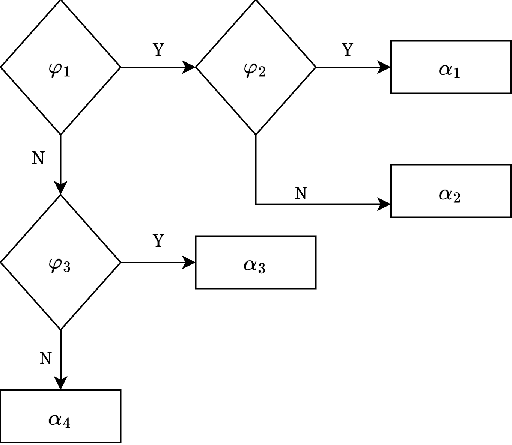
\includegraphics[width=0.5\textwidth]{tgen}
  \caption{T/Gen Example}\label{fig:tgen-example}
\end{figure}

T/Gen's white-box testing approach allows significant reductions in the
number of test cases required for high test-coverage, and has demonstrated
effectiveness in real-world use cases \cite{MillerJAMIA01}. But, it still has
many limitations. Notably:
\begin{itemize}
  \item T/Gen can work with any \CIG{} language, and supports
  a simplified version of \GLIF{}. But, this requires the \CIG{} to
  be re-expressed in T/Gen's simplified language,
  which requires additional effort, especially in cases of languages that differ
    significantly from \GLIF{}. Moreover, the translation effort itself may
    introduce bugs, or, may semantically be different from the original source.
  \item Uncovering additional constraints requires both efforts and expertise.
    As acknowledged in \cite{MillerJAMIA01}, a compromise must be made between
    finding constraints and allowing some redundancy in tests. Moreover,
    introducing constraints can omit certain scenarios, such
    as those dependant on ordering of actions, from being tested.
    Thus, using the tool effectively may require significant effort, depending
    on the complexity of the system under test.
  \item T/Gen utilizes an ad-hoc semantics of \GLIF{}, which may differ from
    that used by \GLIF{} execution engines. Morover, changes to the \GLIF{} language
    over time would also necessitate corresponding updates to T/Gen.
\end{itemize}

\subsection{Verification of Hierarchical Plans}\label{sec:asbru-verification}

In \cite{DuftschmidAIM01}, formal verification of hierarchical plans-based
guidelines is discussed. Although the work specifically focuses on guidelines in
Asbru, it is applicable to other languages that utilize a plan-based approach
to representing \BPGs{}. Recall from \autoref{sec:asbru} that Asbru guidelines
consist of hierarchical plans, where a plan may contain other sub-plans,
thus creating a tree of plans. Leaves of said trees are plans that cannot
be decomposed any further into sub-plans.

A set of eight plan states describe the actual state of the plan during
planning and execution. The following seven conditions define transitions
between aforementioned states:
\begin{enumerate}[label=\arabic*)]
  \item filter-preconditions that hold if an applicable plan cannot be achieved.
  \item setup-preconditions that must hold for an applicable plan to start.
  \item activate-condition that specifies whether plan starts automatically or
    manually.
  \item suspend-conditions that specify when a plan must temporarily halt execution.
  \item abort-conditions that specify when a plan must be stopped unsuccessfully.
  \item complete-conditions that specify successful termination.
  \item reactivate-conditions that enable suspended plans to resume.
\end{enumerate}

The technique described in \cite{DuftschmidAIM01} utilizes static analysis
to ensure plans are \emph{meaningful}, or, verified to not contain well defined
anomalies described in \cite{PreeceJIS94}. Given the hierarchical nature of plans, abnormalities
are classified into:
\begin{enumerate*}[label=(\alph*)]
  \item level 1 that occur within a plan,
  \item level 2 that occur within linked plans,
  \item level 3 that occur at the scale of \BPGs{}.
\end{enumerate*}

In \cite{PreeceJIS94}, a general foundation for reasoning for reasoning
about knowledge bases is provided. A knowledge-base $\mathcal{K} = \mathcal{R}
\cup \mathcal{D}$, where:
\begin{enumerate}
  \item $\mathcal{R}$ is a set rules $\left\{R_1, \dots, R_n\right\}$.
    Rule $R_i$ is an expression of the form of the form
    $L_{i_1} \wedge L_{i_2} \wedge \dots \wedge L_{i_m} \rightarrow R_i$,
    where $L_{i_1}, \dots, L_{i_m}, R_i$ are First-Order Logic literals.
    $\antecedent{R_i} = L_{i_1} \wedge L_{i_2} \dots L_{i_m}$ and $\consequent{R_i} = M_i$.
  \item The set of declarations $\mathcal{D} = \mathcal{G} \cup \mathcal{L} \cup
    \mathcal{C}$ representing the set of goal literals, input literals and
    constraints respectively.
\end{enumerate}
An environment $E$ is defined as a subset of input literals s.t. $E \to
\neg(C\rho)$ for some $c \in \mathcal{C}$ and any substitution $\rho$.
The set of inferrable hypotheses $\mathcal{H}$ is defined as literals
that can be inferred using rules, i.e., for $H \in \mathcal{H}$,
$\exists R \in \mathcal{R}$ s.t. $H = \consequent{R}\rho$ for any
substitution $\rho$. $\left(\mathcal{R} \cup E \right) \vdash H$
denotes that $H$ is inferrable from rule base $\mathcal{R}$ if there
is some environment $E$ s.t. $H$ is the logical consequence of supplying
$E$ to rule $R$.

In \cite{DuftschmidAIM01}, a methodology to transform
an Asbru plans-based guidelines in
Asbru's model of plan states to a rule base $\MPS{}$ is described.
The rules specify the sequence in which the conditions of a plan
are considered. Note that since $\MPS$ encodes the semantics of Asbru,
the translation has to be specified only once.

Next, each plan $P_i$ in the guideline is also encoded as a rule base
$\PC_i$, and the guideline is defined as the rule base $\PC = \PC_1 \cup \PC_2,
\cup \dots \cup \PC_n$. Additionally, the following sets are defined:
\begin{itemize}
  \item $\PlanSet$ -- the set of all plan
  \item $\PatientSet$ -- the set of all patients
  \item $\ConditionSet = \left\{\text{filter}, \text{setup}, \dots,
    \text{complete}\right\}$ corresponding to plan conditions.
  \item $\FinalStateSet = \left\{\text{rejected}, \text{aborted}, \text{completed}\right\}$.
\end{itemize}

The rule base $\MPS{}$ consists of rules encoding the generic model of plan
states. Given parameters $pl$ and $pa$ for a plan and patient respectively,
$\MPS{}$ has rules encoding states such as:
\begin{itemize}
  \item $\Considered(pl)$ encodes the starting state of each plan.
  \item $\Considered(pl,pa) \wedge \filter(pl,pa) \to \possible(pl,pa)$
    encodes the condition that a plan with filter conditions satisfied
    is possible for execution.
\end{itemize}

Next, Asbru plan $i$ in the guideline need to be transformed into
its corresponding rule base $PC_i$. For instance, a plan for
treatment of non-insulation dependandant gestation diabetes militus,
in patients with normal blood glucose levels, called GDM-TYPE-II,
contains rules of the form:
\begin{itemize}
  \item $\text{Female}(pa) \wedge \text{Pregnant}(pa) \to \filter(\text{GDM-TYPE-II}, pa)$
    encodes that pregnant female patients should be considered for the plan.
  \item $\text{Activate}(\text{GDM-TYPE-II}, pa)$ encodes that the plan should
    be automatically activated.
  \item $\text{State}(\text{blood-glucose-high}, pa) \to \text{suspend}(\text{GDM-TYPE-II},pa)$
    encodes that if the plan be suspended in case of high blood sugar.
  \item $\text{State}(\text{blood-glucose-normal}, pa) \to \text{reactivated}(\text{GDM-TYPE-II},pa)$
    similary encodes that the guideline be reactivated when blood sugar returns
    to normal.
\end{itemize}

Once the guideline has been encoded as a rule base using the above mentioned
transformation, important properties can be checked against the rule base.
For instance, conditions in a plan must be satisfiable in order to
have an effect on the plan. Formally, this is equivalent to checking
all rules in the rule base are \emph{fireable}. If a condition,
such as $\text{Male}(pa) \wedge \text{Pregnant}(pa) \to \filter(\text{plan}, pa)$
contains a conjunction that cannot be satisfied, then it does not contribute
to the plan's execution, and, is not \emph{meaningful}.

The work methodology describe above represents significant progress towards
verification of meaningful properties on real guidelines. But, the methodology
also has limitations, such as:
\begin{itemize}
  \item It only works for certain pre-defined anomalies.
  \item Expressing hierarchical plans in Asbru as knowledge-bases from
    \cite{PreeceJIS94} utilizes an ad-hoc semantics of Asbru.
  \item Any update to Asbru would necessitate corresponding updates to
    the verification tool.
\end{itemize}

\subsection{Model-driven Development and Verification}\label{sec:mda-verification}

In \cite{PerezJBI10}, the authors present a comprehensive approach
to development and verification of guidelines, called the Model Driven
Architecture (\MDA{}). Instead of
utilizing a domain specific language, they choose to model \BPGs{}
as UML Statecharts \cite{OMGSpecUrl}. The choice is motivated by
the fact that Statecharts have been used to build systems in diverse
domains such as Air Traffic Control \cite{WhittleICSE02} and biology
\cite{EfroniGR03}.

The development and verification methodology has several steps.
First, software engineers and experts in medicine collaborate
express the guideline using Statecharts. Next, patterns
representing common errors in guidelines are utilized to
write specifications for the guidelines. The
the Statecharts code is automatically translated to PROMELA,
the language of the SPIN model checker \cite{MikkISFST98} for verification.
To turn the verified Statechart guidelines into a \CDSS{}, the
\MDA{}-based approach includes tools that translate the Statecharts into
executable Java code that is combined with additional infrastructure to
obtain a functioning \CDSS{}.

\subsubsection{Property Specification}

In \cite{PerezJBI10}, the authors deal with
medical properties, or properties that are not implementation-related,
dealing with aspects such as  medical parameters, \HCP{} actions,
and overall guideline intentions. As specifying properties
requires expertise and a mathematical background. The \MDA{}
approach includes a number of common patterns applicable
to all guidelines that can be
used as templates for writing actual properties. Thus,
through the use of these patterns, the authors attempt
to enable even non-experts to use the \MDA{} verification
methodology.

Property patterns in the \MDA{} verification methodology
are based on existing work on simplifying verification for
concurrent and reactive systems through safety and liveness patterns
that contain informal descriptions of the property and
well-defined translations to widely used temporal logics such
as computation tree logic (\CTL{}) and linear temporal logic (\LTL{})
\cite{DwyerFM98,DwyerICSE98,BitschSAFECOMP01,RyndinaThesis05}.

To ensure that that patterns presented under the \MDA{} framework
cover a wide spectrum of possible properties, the authors
collected properties relevant to \BPGs{} from literature, and attempted
to represent them using specification patterns proposed by Dwyer et al.
in \cite{DwyerFM98}. However, they realized that Dwyer patterns
were insufficient to represent all properties of interest. To
address this the authors:
\begin{enumerate*}[label=(\alph*)]
  \item utilized an expanded pattern representation schema
    proposed by Ryndina et al in \cite{RyndinaThesis05}, and,
  \item proposed a new patterns to encompass all desired properties.
\end{enumerate*}
This expanded representation schema enables the authors to represent
useful and complex properties, at both local and global scopes, and
dealing with both safety (something bad never occurs) and liveness
(always something desirable eventually occurs).

In \cite{PorresECBS08}, \MDA{}
is used to implement and analyze the
\IRC{} guideline for management of infections due
to intravenous catheters. The verification process revealed
several inconsistencies, which were fixed. Moreover, the \CDSS{}
was shown to satisfy several important properties. Several
important patterns were identified during the verification process,
which are also applicable to other guidelines. For instance,
it is important to ensure
that if an empirical treatment has not been ordered, then
it is not removed later on. This is identified as
an instance of the absence-after pattern, and can
be represented by the \LTL{} formula
$\eventually\neg\left(\text{removeTreatment} == \text{Empirical} \to
\text{beginTreatment} == \text{Empirical}\right)$.
Another pattern of interest is possible-existence, stating that,
starting from a certain patient
state leads to a desired guideline-based outcome. For instance,
in case of the \IRC{} guideline, the authors verified that
starting from clinical test results that were not indicative of
\IRC{}, it is never possible to reach a state where \IRC{} is indicated.
Thus, the verification process revealed both inconsistencies in the guidelines
and ensured that other desired properties are satisfied \cite{PerezJBI10}.

The \MDA{} approach has several strengths. Notably:
\begin{itemize}
  \item The approach has been used to implement real-world
    systems and verify important properties against them,
    as demonstrated in \cite{PorresECBS08}.
  \item Utilizes existing work in modeling large concurrent
    systems as Statecharts, instead of implementing a \DSL{} from
    scratch, allowing existing tools for visualization to be used.
  \item Unlike other approaches, emphasis is given to ensuring
    that expertise in mathematics is not needed for verification,
    through the use of property patterns for property specification,
    and automated translations of the \BPG{} and property to PROMELA
    for verification using SPIN.
\end{itemize}

However, the approach also has some limitations. First, in order to execute the
Statecharts-based \BPG{} in a \CDSS{}, a translation from the OMG Systems
Modeling Language \cite{OMGSpecUrl} to Java is utilized, and for
verification via SPIN, a translation to PROMELA is utilized. Thus, it
is possible for the translations to diverge from the underlying \BPG{}
in the OMG Systems Modeling Language. This can have serious
consequences, as verification results may not be satisfied by the actual
implementation. Thus, even though utilizing specification patterns
may enable non-experts in verification to verify properties PROMELA model,
expertise in formal reasoning may be required to ensure that the model
corresponds to the original \BPG{} and the corresponding Java code.
Second, only a subset OMG Systems Modeling Language is supported
by the tools in \cite{PerezJBI10,PorresECBS08}, and the translation
are tied to a particular version of the language. Supporting newer
versions of the language and updates to the language would require
corresponding updates to the entire toolchain. Finally, while several
important properties can be established using model checking in SPIN,
supporting other techniques such as symbolic execution or deductive
verification would require similar translation to other languages, which
would further require increase the chances of the many translations
diverging from the underlying \BPG{}.

\section{Discussion}\label{sec:related-work-discussion}

In \autoref{chapter:hurdles-cdss-adoption}, we discussed several
challenges that limit wider \CDSSs{} uptake in practice. The
approaches discussed in this chapter make significant headway into
addressing said challenges. These challenges (Cs) were concisely
described in \autoref{sec:hurdles-cdss-adoption} as:
\begin{enumerate}[label=C\arabic*.]
\itemsep0.0em
\item Absence of systematic ways of \emph{validating content}
in a \emph{reliable}, \emph{accessible} and \emph{updateable} manner.
\item Lack of \emph{reliable}, \emph{shareable} \CDSS{} content
that can be easily adopted across healthcare organizations and their (Information
Technology) \IT{} systems.
\item Technical difficulties of sharing due to \emph{need for
  adaptation} to diverse Electronic Health Records (\EHR) systems.
\item \emph{Suboptimal} User Interfaces (\UIs), implementation choices and
workflows.
\end{enumerate}

In \autoref{sec:addressing-hurdles}, we outlined major
themes behind addressing aforementioned challenges. We briefly
recap those themes here:

\paragraph{Implementation-Specification Gap}

Textual \BPGs{} are often written by medical experts, but,
the translation into an executable computer program is
provided is performed by software developers and knowledge
engineers who typically lack the necessary expertise to ensure
medical knowledge is correctly encoded. The textual \BPG{} is
utilized as a functional specification to develop the \CDSSs{}.
This make it possible for the specification to diverge from the
implementation, leading to an implementation-specification gap.

\DSLs{} for computer-interpretable guidelines aim to eliminate
the aforementioned gap by emphasizing \HCP{} comprehensibility,
thereby enabling the \CIG{} to also serve as the guideline's
textual description, eliminating the implementation-specification gap,
and are vital to developing trusted guidelines with validated content.

\paragraph{Formal Semantics}

In order to utilize formal methods to ensure \CDSS{} correctness,
the underlying language utilized to express guidelines must have
a complete, well-defined formal semantics \cite{ShaharAMIA96}. The
semantics can then be utilized to implement tools for execution and analysis,
to support a development of verified guidelines.

\paragraph{Formal Analysis Tools}

A comprehensive suite of formal analysis tools---model checkers,
symbolic execution engines, and deductive verifiers---is essential for
developing systems with desired safety properties.
Additionally, it is crucial to keep these tools updated as the language evolves.
As \DSLs{} for computer interpretable guidelines adapt
to lessons from implementing best practice guidelines (\BPGs{}),
mechanisms must be in place to update all relevant tools, and not just
ones needed for immediate use, such as execution engines.

\paragraph{Holistic Safety}

Ensuring that computer interpretable guidelines
meet desired correctness properties is crucial,
but it is equally important to ensure that tools used
to execute and analyze said guidelines themselves are correct,
as bugs can compromise patient safety.
We use the term \say{holistic safety} to refer to approaches that
have a complete formal semantics and a comprehensive suite of execution
and formal analysis tools derived using them,
each with correctness guarantees.

  \begin{table}[b!]
    \begin{tabularx}{\textwidth}
   {>{\centering\arraybackslash}X
   || >{\centering\arraybackslash}X
   | >{\centering\arraybackslash}X
   | >{\centering\arraybackslash}X
   | >{\centering\arraybackslash}X
 }
                                    & Implementation-Specification Gap & Complete Formal Semantics & Formal Analysis Tools & Holistic Safety  \\
    Arden Syntax                    & $\greencheck$                    & $\redcross$               & $\redcross$           & $\redcross$ \\
    DILLEMA                         & $\greencheck$                    & $\redcross$               & $\redcross$           & $\redcross$ \\
    \GEODECM{}                      & $\greencheck$                    & $\redcross$               & $\redcross$           & $\redcross$ \\
    EON                             & $\greencheck$                    & $\redcross$               & $\redcross$           & $\redcross$ \\
    \GLIF{}                         & $\greencheck$                    & $\redcross$               & $\redcross$           & $\redcross$ \\
    Asbru                           & $\greencheck$                    & $\circ$                   & $\greencheck$         & $\redcross$ \\
    PROforma                        & $\greencheck$                    & $\greencheck$             & $\redcross$           & $\redcross$ \\
    \GLARE                          & $\greencheck$                    & $\circ$                   & $\circ$               & $\circ$     \\
    \GPROVE{}                       & $\greencheck$                    & $\greencheck$             & $\redcross$           & $\redcross$ \\
    HELEN                           & $\greencheck$                    & $\redcross$               & $\redcross$           & $\redcross$ \\
    PRODIGY                         & $\greencheck$                    & $\redcross$               & $\redcross$           & $\redcross$ \\
    SAGE                            & $\greencheck$                    & $\redcross$               & $\redcross$           & $\redcross$ \\
    Hierarchical Plans              & $\redcross$                      & $\circ$                   & $\greencheck$         & $\circ$     \\
    \MDA{}                          & $\redcross$                      & $\redcross$               & $\greencheck$         & $\redcross$ \\
  \end{tabularx}
  \caption{Comparison of Existing Approaches}\label{table:dsl-comparison}
  \end{table}


Next, we discuss how approaches discusses in this chapter compare
w.r.t. aforementioned themes. In \autoref{table:dsl-comparison}, we
show whether each approach fully addressed ($\greencheck$), partly
addresses $\circ$ or doesn't address ($\redcross$) issues related
to said theme. For example, all $\DSLs{}$ specifically designed
with comprehensibility to \HCPs{} in mind eliminate the
implementation-specification gap, as guidelines expressed using these \DSLs{}
can serve as both the \HCP{}-readable textual representation, and
its computable translation as a \CDSS' \BPGLogic{}.

The outlined languages can be categorized into either \DSLs{} for \CIGs{},
or, general ones for building concurrent systems. For instance,
the Arden Syntax (\autoref{sec:arden-syntax})
was among the first languages specifically designed to be
comprehensible to \HCPs{}, and is still widely used for expressing medical
knowledge. But, it's designed for simpler, independent guidelines, and
is unsuitable for complex workflows. Other approaches
such DILLEMA (\autoref{sec:dilemma}) and \GEODECM{}
(\autoref{sec:geodecm}) enabled expressing more complex guidelines,
and modular architectures that integrate with diverse systems.
However, since these were among the earliest attempts at building modular \CDSSs{},
functionality was prioritized over formal correctness.

EON (\autoref{sec:eon}) switched from small, modular and
independent guidelines from Arden Syntax to more complex,
tightly coupled state machines-based representation to enable modeling
interdependent workflows. Similarly, \GLIF{} (\autoref{sec:glif}) borrowed experiences from
EON, \GEODECM{} and Arden Syntax to facilitate modeling complex workflows.
The design and implementation of \GLIF{} was particularly influenced
by the motivation to allow \GLIF{}-based guidelines to be easily shared
between medical establishments. Similarly, Prodigy (\autoref{sec:prodigy})
tackled \CDSSs{} challenges encountered in practice, such as diversity in
 data sources, and their unreliability, while \SAGE{} (\autoref{sec:sage})
attempted to integrate with existing digital workflows as seamlessly as
possible. It's important to note that these approaches demonstrated that computerized decision support
systems can both
\begin{enumerate*}[label=(\alph*)]
  \item manage complex guidelines with interdependent concurrent tasks, and,
  \item be modular and portable to accommodate hospital-specific customizations,
    and integrate with their \EHR{} systems.
\end{enumerate*}
But, system safety and correctness wasn't a challenge that these approaches
were directly attempting to address.
Thus, they lack a complete formal semantics, and a suite of tools accompanying
analysis tools.

The need for a complete formal semantics to enable development of tools for
execution and analysis of guidelines has already been recognized by several
approaches. For instance, the lack of ways to systematically analyze guidelines
in HELEN (\autoref{sec:helen}), and an execution engine based on ad-hoc
semantics has already been recognized as a limitation of the framework.
 PROforma (\autoref{sec:proforma}), and
Asbru (\autoref{sec:asbru}) attempt to address this by having formal
semantics, albeit incomplete semantics, that are intended to guide tool
development. The Asbru language has an incomplete, but formal
\SOS{} paper-based semantics. But, according to the authors of
\cite{SuttonAMIA03}, it is insufficient for developing tools for the language.
Despite its incompleteness, Asbru language's semantics has served as a calculus for deductive verification
using KIV, as described \autoref{sec:kiv-verification}.
Along similar lines, a formal but incomplete paper-based semantics
of the PROforma language is
presented in \cite{SuttonAMIA03}, with the aim of serving as a manual for
developing PROforma tools. Both approaches take significant steps towards using
recognizing formal semantics, and using them in some ways
to establish \CDSS{} safety. But, the support for formal analysis is very
limited. Moreover, the tools aren't directly derived
from the semantics, and need to be updated every time the language evolves,
which can potential lead to a divergence between the official semantics, and
the ones utilized by said tools.

Approaches such as \GLARE{} (\autoref{sec:glare}) and \GPROVE (\autoref{sec:gprove}), also have tools that allow complex guidelines to
be both modeled and analyzed, but said tools are based on ad-hoc language
semantics. For instance, GLARE{} provides mechanisms to check
for inconsistencies in the guidelines such as unintended cyclic
behavior, choices without alternative options, and actions
with unsatisfiable temporal constraints. Notably, \GPROVE{}
has capabilities to enable a-posteriori compliance checking, i.e., checking whether a log
generated during execution indicates adherence (or lack thereof) to the guideline.
To this end, \GOSPEL{} (the language for expressing guidelines in \GPROVE{})
is translated to Sciff -- a constraint logic programming framework.
But, both \GLARE{} and \GPROVE{} lack formal semantics. \GLARE{}'s analysis
and \GPROVE{}'s Sciff translator and execution trace generator are based on
ad-hoc semantics of the underlying languages, making it possible for the
analysis results to not hold on the actual programs.

Next, we consider approaches that rely on general solutions for building
concurrent systems for building and analyzing \CDSSs{}. The verification methodology
defined in \autoref{sec:asbru-verification} utilizes foundational work in
reasoning with knowledge bases to reason about Asbru guidelines. But, it
can work with any language that utilizes a plan-based approach to
represent guidelines. Similarly, the \MDA{}-based approach relies
on guidelines expressed as Statecharts in the OMG systems modeling language.
The OMG Statecharts are then translated to PROMELA for verification using the SPIN,
and into executable Java code for use as a \CDSS{}.
For convenience, we refer to the representation that guidelines are directly
encoded in as \say{\HCP{}-friendly}, and the translated representation
used for analysis as \say{analysis-friendly}.
For instance, for the \MDA{}-based approach described in \autoref{sec:mda-verification}, we refer to Statecharts as the \say{\HCP{}-friendly}
, and the translated PROMELA code as \say{analysis-friendly}.
Thus, for both these approaches:
\begin{enumerate*}[label=(\alph*)]
  \item These exists a specification-implementation gap, where the
    \say{HCP-friendly} guideline serves as the specification, and the
    translated PROMELA or Java code serves as the implementation.
  \item the translation from the \say{\HCP{}-friendly} representation to
    an \say{executable} one, or a \say{analysis-friendly} is typically based on an
    ad-hoc semantics of the \say{\HCP{}-friendly} language. Thus, even though
    the \say{analysis-friendly} representation may have well-defined formal
    semantics, the results of analysis may not hold on the \say{\HCP{}-friendly}
    notation.
\end{enumerate*}
Moreover, in case of the \MDA{}-based approach, the \say{\HCP{}-friendly}
notation is translated to Java for execution. But, as the Java and
PROMELA translations are not proven to be equivalent, it is possible for
the results of model checking through SPIN may not be applicable to the
corresponding Java code.


%\begin{center}
%\renewcommand{\arraystretch}{0.5}
%\setlength\extrarowheight{-9pt}
%\end{center}



%The verification is performed bottom-up -- from the leaves of the hierarchical
%plan to the eventual root representing the guideline.
%In \cite{PreeceJIS94},
%the authors describe verification of anomalies for knowledge bases by modeling
%a knowledge base as a union of a rule base and set of declarations, where rules are
%statements that define transitions, and
%the set of declarations comprising of possible outputs,
%the input vocabulary and constraints.
%By modeling Asbru plans as a knowledge-base, the authors are able to
%utilize existing techniques for checking anomalies from \cite{PreeceJIS94}
%to Asbru plans.



